%Beamer class
\documentclass{beamer}

\usepackage[czech]{babel}
\usepackage[utf8]{inputenc}
\usepackage{fontenc}
\usepackage{tgheros}
\usepackage{array}
\usepackage{color}
\usepackage{hyperref}

\usetheme{AnnArbor}
\usecolortheme{crane}


\title[Realizace prototypu]{Realizace prototypu}
\subtitle[KEO] {Konstrukce a realizace elektronických obvodů}
\author[Brejcha]{\texorpdfstring{Michal Brejcha\newline\url{brejcmic@fel.cvut.cz}}{Michal Brejcha}}
\institute[ČVUT]{ČVUT v Praze, FEL}
\date[Praha, 2024]{Praha, 2024}

%------------------------------------------------------------------------------
%Konstanty a definice
%------------------------------------------------------------------------------
\newtheorem{myDef}{}

\begin{document}
%------------------------------------------------------------------------------
%Uvodni slajd
%------------------------------------------------------------------------------
\frame{\titlepage}

\begin{frame}
\frametitle{Obsah} 
\tableofcontents
\end{frame}

\AtBeginSection[]
{
  \begin{frame}
    \frametitle{Téma}
    \tableofcontents[currentsection]
  \end{frame}
}

%------------------------------------------------------------------------------
%Návrh
%------------------------------------------------------------------------------
\section{\texorpdfstring{Simulace obvodu}{Simulace obvodu}}
%------------------------------------------------------------------------------
  \begin{frame}
    \frametitle{Ukázka simulačního SW}
    
		Volně stažitelné nástroje:
		
		\begin{itemize}
			\item \textbf{LTSpice:} \\ \url{https://www.analog.com/en/resources/design-tools-and-calculators/ltspice-simulator.html}
			\item \textbf{Micro-Cap 12:} \\ \url{https://micro-cap.informer.com/12.0/}
			\item \textbf{Qucs-S:} \\ \url{https://ra3xdh.github.io/}
		\end{itemize}
    
  \end{frame}
%------------------------------------------------------------------------------
  \begin{frame}
    \frametitle{LTSpice}
    
		\begin{center}
			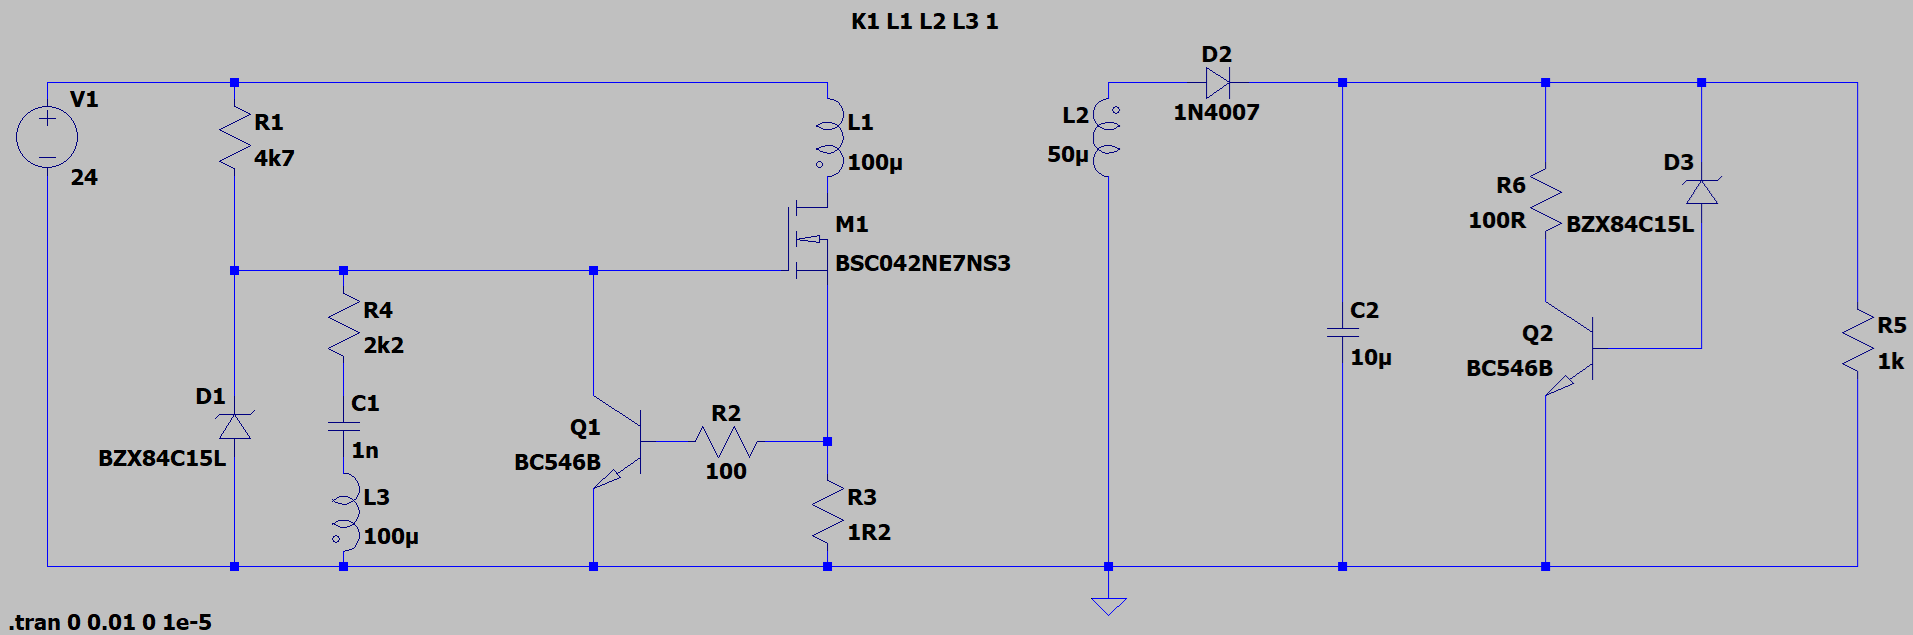
\includegraphics[width=0.95\textwidth]{obr/LTSpice.png} 
		\end{center}
		
		
		\begin{itemize}
			\item Jednoduché ovládání,
			\item málo obsáhlé knihovny,
			\item vhodné pro simulaci měničových struktur a filtrů.
		\end{itemize}
    
  \end{frame}
%------------------------------------------------------------------------------
  \begin{frame}
    \frametitle{Micro-Cap 12}
    
		\begin{center}
			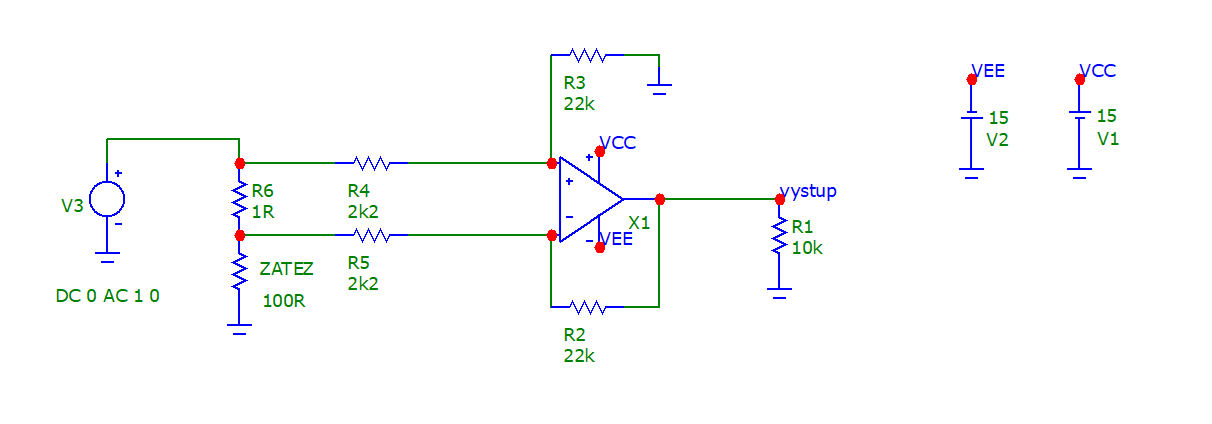
\includegraphics[width=0.95\textwidth]{obr/microcap12.png} 
		\end{center}
		
		
		\begin{itemize}
			\item Trýznivé ovládání,
			\item obsáhlé knihovny,
			\item možnost dynamické simulace,
			\item vhodné pro simulaci obvodů s integrovanými obvody.
		\end{itemize}
    
  \end{frame}
%------------------------------------------------------------------------------
  \begin{frame}
    \frametitle{Qucs-S}
    
		\begin{center}
			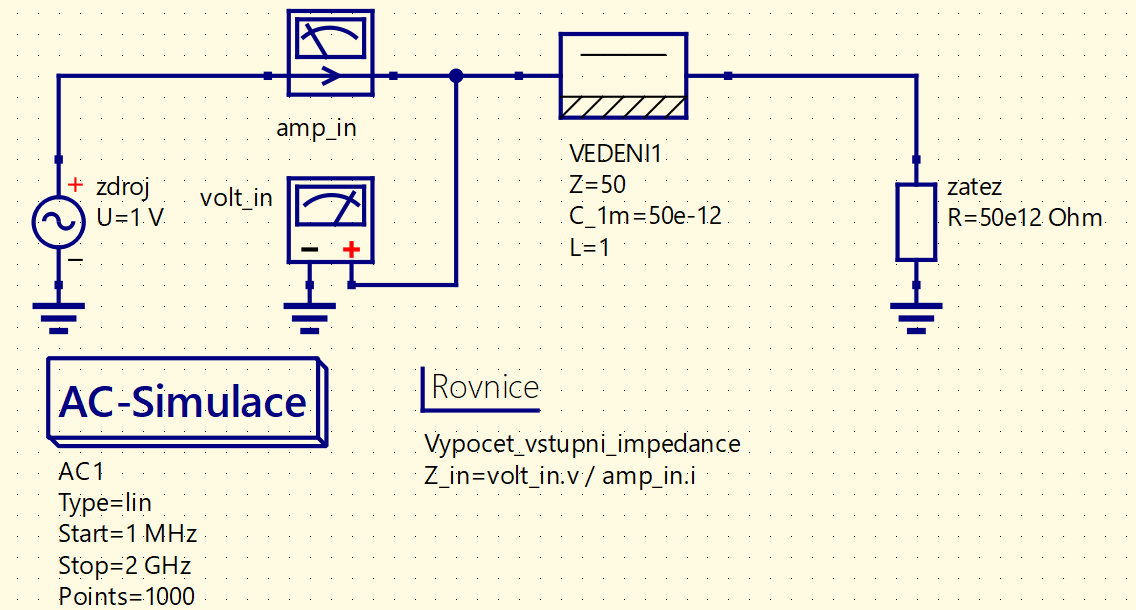
\includegraphics[width=0.7\textwidth]{obr/qucs-s.png} 
		\end{center}
		
		
		\begin{itemize}
			\item Jednoduché ovládání,
			\item málo obsáhlé knihovny,
			\item snadná tvorba podobvodů,
			\item vhodné pro modelování obvodů.
		\end{itemize}
    
  \end{frame}
	
%------------------------------------------------------------------------------
% Dispozice obvodu
%------------------------------------------------------------------------------
\section{\texorpdfstring{Dispozice obvodu}{Dispozice obvodu}}
%------------------------------------------------------------------------------
  \begin{frame}
    \frametitle{Rozmístění obvodových částí}
    
			\begin{tabular}{ p{55mm} p{55mm} }
				\begin{center}
					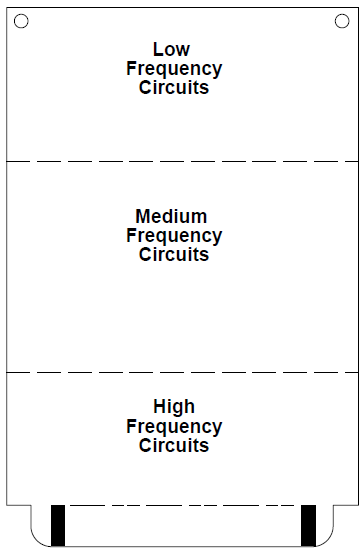
\includegraphics[width=0.35\textwidth]{obr/dispozice.png} 
				\end{center} &
				
				\begin{itemize}
					\item vf obvody nejblíže konektoru,
					\item úprava DC napětí bude nejdále.
				\end{itemize}
			\end{tabular}
    
  \end{frame}
%------------------------------------------------------------------------------
  \begin{frame}
    \frametitle{Propojení napájených částí}
		
    \begin{tabular}{ p{55mm} | p{55mm} }
				\hline
				\begin{center}
					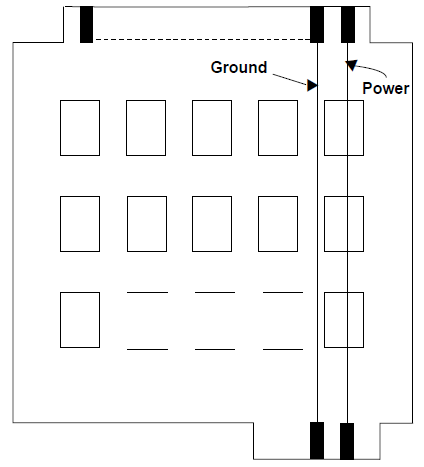
\includegraphics[scale=0.45]{obr/privod_napajeni_nevhodne.png} 
				\end{center} &
				
				\begin{center}
					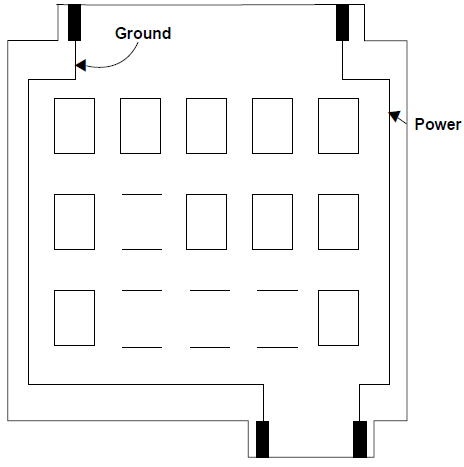
\includegraphics[scale=0.45]{obr/privod_napajeni_vhodne.png} 
				\end{center} \\
				
				Méně vodné z hlediska rušení & Lepší, ale vzniká větší smyčka \\ 
				\hline
			\end{tabular}
			
			
			\begin{itemize}
			  \item Propojujeme dvě strany DPS
				\item mimo prostor aktivních obvodů.
			\end{itemize}
			
  \end{frame}
	
%------------------------------------------------------------------------------
	\begin{frame}
    \frametitle{Přívod napájení k prvkům}  
		
			\begin{tabular}{ p{55mm} p{55mm} }
				\begin{center}
					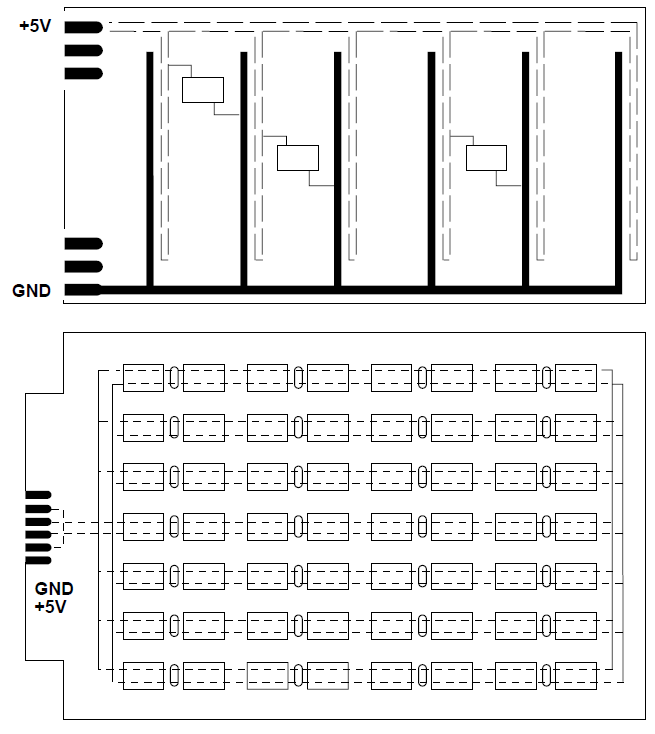
\includegraphics[width=0.5\textwidth]{obr/rozvod_napajeni_ne_ano.png} 
				\end{center} &
				
				\begin{enumerate}
					\item Hřebenová struktura = nevhodná
					
					\begin{itemize}
						\item Velké smyčky,
						\item galvanická vazba přes T uzly.
					\end{itemize}
					
					\item Řádková struktura = lepší
					
					\begin{itemize}
						\item Rozvod v blízkosti zdroje,
						\item malé smyčky,
						\item krátké přívody snižují galvanickou vazbu.
					\end{itemize}
					
					\item Referenční plochy = nejlepší
						\begin{itemize}
							\item Nízká impedance propojení,
							\item malé vazby.
						\end{itemize}
				\end{enumerate}
			\end{tabular}
    
  \end{frame}
%------------------------------------------------------------------------------
\subsection{\texorpdfstring{Prototypová deska s prokovy}{Prototypová deska s prokovy}}
%------------------------------------------------------------------------------
  \begin{frame}
    \frametitle{Prototypová deska s prokovy (pady) - perfboard}
    \begin{center}
      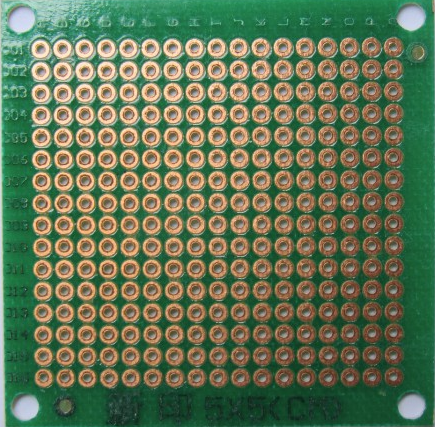
\includegraphics[width=0.5\textwidth]{obr/perfBoard_bot.png}
    \end{center}
  \end{frame}
%------------------------------------------------------------------------------
  \begin{frame}
    \frametitle{Prototypová deska s prokovy (pady) - perfboard}
    \begin{center}
      \includegraphics[width=\textwidth]{obr/teplomer1}
    \end{center}
  \end{frame}
%------------------------------------------------------------------------------
  \begin{frame}
    \frametitle{Prototypová deska s prokovy (pady) - realizace prototypu}
    \begin{center}
      \includegraphics[width=\textwidth]{obr/teplomer2}
    \end{center}
  \end{frame}
%------------------------------------------------------------------------------
\subsection{\texorpdfstring{Prototypová deska s pásky}{Prototypova deska s pasky}}
%------------------------------------------------------------------------------
  \begin{frame}
    \frametitle{Prototypová deska s pásky - stripboard}
    \begin{center}
      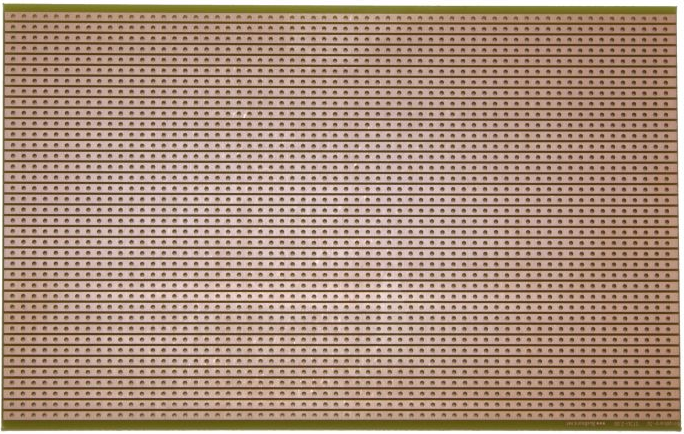
\includegraphics[width=0.8\textwidth]{obr/stripBoard_bot.png}
    \end{center}
  \end{frame}
%------------------------------------------------------------------------------
  \begin{frame}
    \frametitle{Prototypová deska s pásky - realizace prototypu}
    \begin{center}
      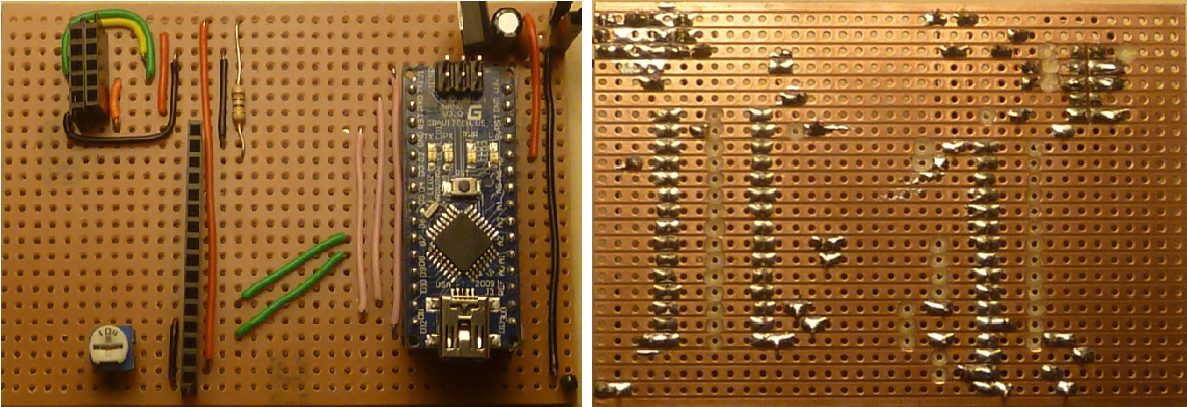
\includegraphics[width=\textwidth]{obr/stripBoard_prot.png}
    \end{center}
  \end{frame}
%------------------------------------------------------------------------------
  \begin{frame}
    \frametitle{Prototypová deska s pásky - návrh}
    \begin{center}
      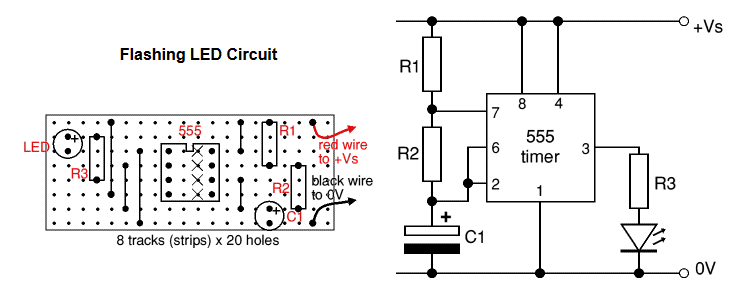
\includegraphics[width=\textwidth]{obr/stripBoard_desgn.png}
    \end{center}
  \end{frame}
	
%------------------------------------------------------------------------------
% Prezentace
%------------------------------------------------------------------------------
\section{\texorpdfstring{Prezetace zadání}{Prezentace zadani}}
%------------------------------------------------------------------------------
  \begin{frame}
    \frametitle{Vlastnosti prezentace}
		
		\begin{enumerate}
			\item Forma:
				\begin{itemize}
					\item Maximálně 3 slajdy nebo popis na maximálně 2 strany A4,
					\item odevzdávejte jako PDF soubor do moodle,
					\item Obsah: co chci dělat, jaké jsou parametry obvodu nebo jaké očekávám, referenční zapojení.
				\end{itemize}
			\item Důvod:
				\begin{itemize}
					\item Seznámení ostatních s projektem, který chcete realizovat $\Longrightarrow$ nutnost prezentace.
					\item Odevzdání prezentace do moodle zajistí, že vyučující bude mít přehled o tématech projektů.
				\end{itemize}
		\end{enumerate}
		\vspace{4mm}

  \end{frame}
%------------------------------------------------------------------------------
  \begin{frame}
    \frametitle{Moodle}
    \begin{center}
      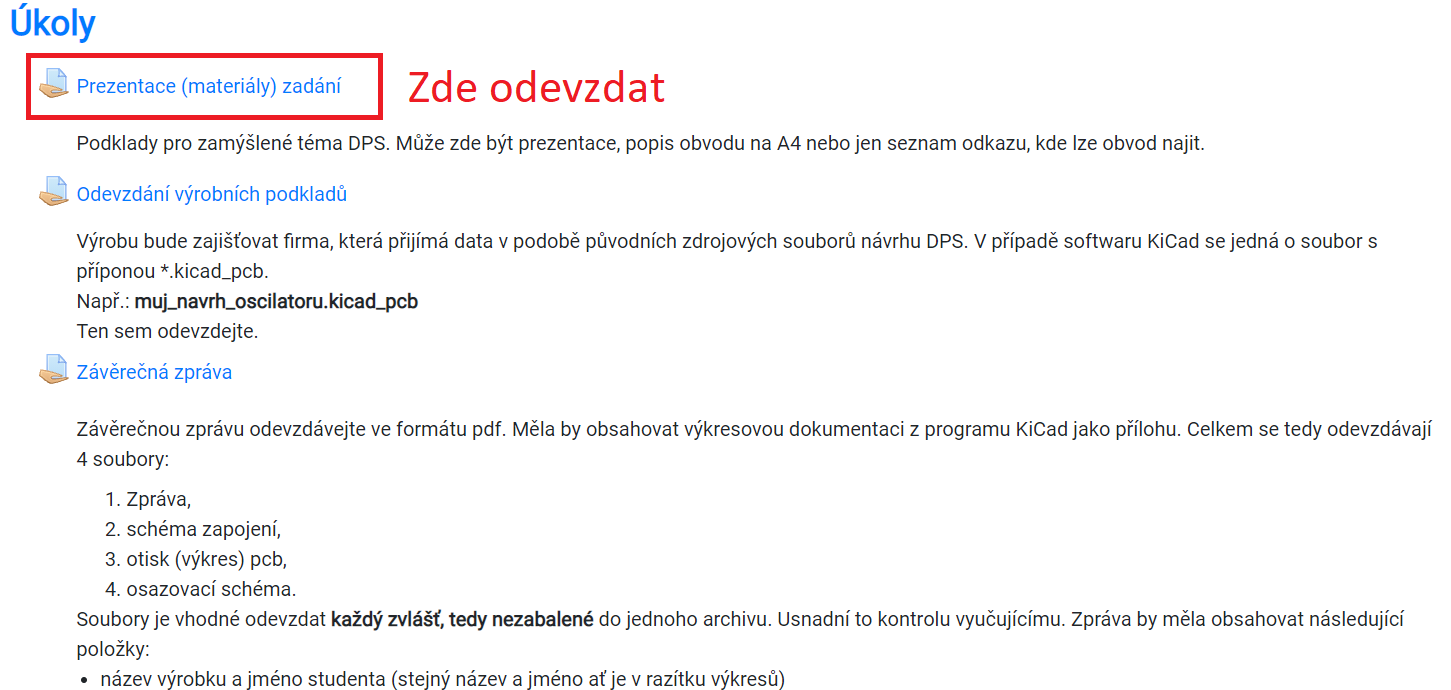
\includegraphics[width=\textwidth]{obr/moodle_ukoly.png}
    \end{center}
  \end{frame}
%------------------------------------------------------------------------------
	\begin{frame}
    \frametitle{Ukázka prezentace - Vojtěch Nydrle}
		
		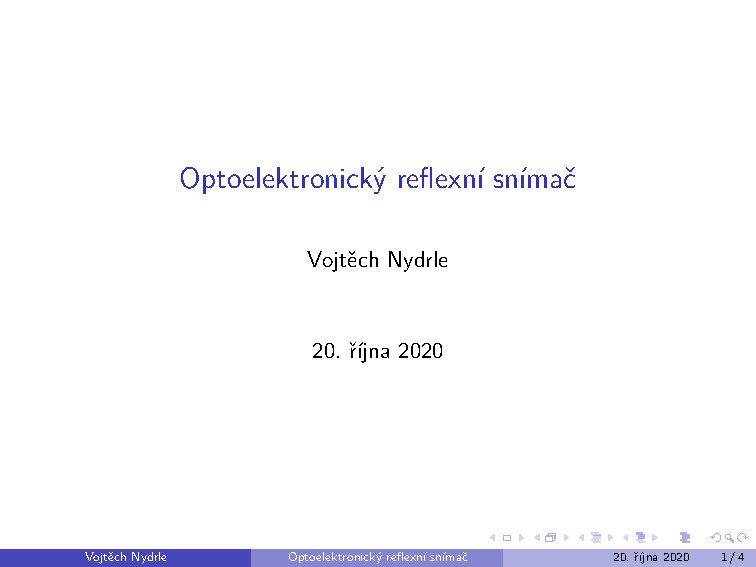
\includegraphics[page=1,width=0.9\textwidth]{pdf/prezentace_Vojtech_Nydrle.pdf}
	
	\end{frame}
%------------------------------------------------------------------------------
	\begin{frame}
    \frametitle{Ukázka prezentace - Vojtěch Nydrle}
		
		\includegraphics[page=2,width=0.9\textwidth]{pdf/prezentace_Vojtech_Nydrle.pdf}
	
	\end{frame}
%------------------------------------------------------------------------------
	\begin{frame}
    \frametitle{Ukázka prezentace - Vojtěch Nydrle}
		
		\includegraphics[page=3,width=0.9\textwidth]{pdf/prezentace_Vojtech_Nydrle.pdf}
	
	\end{frame}
%------------------------------------------------------------------------------
	\begin{frame}
    \frametitle{Ukázka prezentace - Vojtěch Nydrle}
		
		\includegraphics[page=4,width=0.9\textwidth]{pdf/prezentace_Vojtech_Nydrle.pdf}
	
	\end{frame}
%------------------------------------------------------------------------------
	\begin{frame}
    \frametitle{Ukázka stránky A4 - Šimon Hykl}
		
		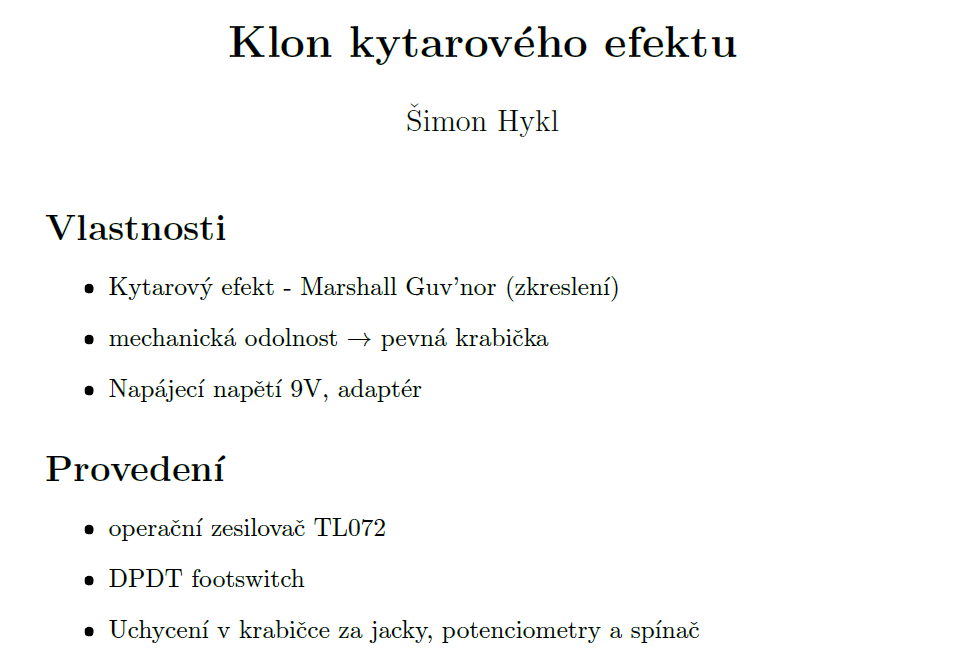
\includegraphics[scale=0.5]{obr/A4_Hykl1.png}
	
	\end{frame}
%------------------------------------------------------------------------------
	\begin{frame}
    \frametitle{Ukázka stránky A4 - Šimon Hykl}
		
		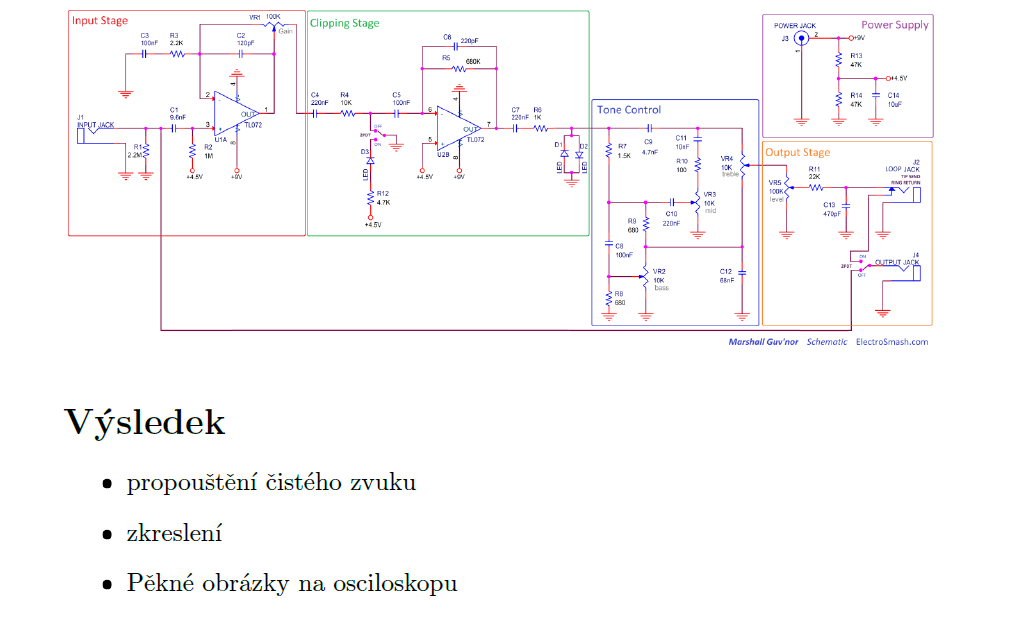
\includegraphics[scale=0.5]{obr/A4_Hykl2.png}
	
	\end{frame}
%------------------------------------------------------------------------------
  \begin{frame}
    \frametitle{Co bude příště}
    
    \begin{itemize}
      \item Prezentace vašich obvodů,
			\item rozhodneme, kterou část obvodu by bylo vhodné odzkoušet jako prototyp,
      \item příprava na KiCAD - kde ho stáhnout, instalace atd.
    \end{itemize}
    
  \end{frame}
%------------------------------------------------------------------------------
\end{document}